

\documentclass{beamer}
\beamertemplatenavigationsymbolsempty

\usepackage[utf8]{inputenc}         % Input encoding (allow direct use of special characters like "ä")
%\usepackage[english]{babel}
\usepackage[ngerman]{babel}
\usepackage[T1]{fontenc}
\usepackage[automark]{scrpage2} 	 % Schickerer Satzspiegel mit KOMA-Script
\usepackage{setspace}           	 % Allow the modification of the space between lines
\usepackage{caption}

\captionsetup[figure]{labelformat=empty}

\usepackage{pdfpages}
% Um .eps Files einzubinden 
\usepackage{epstopdf} 

\AtBeginSection[]
{
  \begin{frame}
    \frametitle{Table of Contents}
    \tableofcontents[currentsection]
  \end{frame}
}

\setbeamercovered{transparent}
\beamertemplatenavigationsymbolsempty
\setbeamertemplate{footline}[frame number]

\usetheme{Madrid}

\title[Seminar]{IT-Sicherheit Seminar}
\subtitle[Remailer]{Remailer: Typ-I bis Typ-III}
\author[M. McCreight]{Mervyn McCreight}
\institute[FH-Wedel]{FH-Wedel}

\subject{Remailer}
\keywords{Remailer, IT, Security, Anonymous, Pseudonymous}

\begin{document}

\frame{\titlepage}

\section{Motivation}
\begin{frame}
	\frametitle{Warum Remailer?}
	
	\visible<1-2>{
	\begin{exampleblock}{Sitzung}
	\begin{columns}[T]
		\begin{column}{2.5cm}
			\vspace{-.3cm}
			\centering
				\begin{figure}
					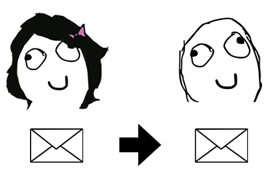
\includegraphics[height=2.5cm]{bilder/modell.jpg}
				\end{figure}
		\end{column}
		\begin{column}{7cm}	
			\centering
			\begin{itemize}	
				\item Alice möchte Bob Nachricht senden
				\item Normal: Schutz des Inhalts
				\item Jetzt: Schutz der Identitäten
			\end{itemize}
		\end{column}
	\end{columns}
	\end{exampleblock}
	}
	
	\invisible<1> {
	\begin{alertblock}{Angreifer Eve möchte Ziele gefährden}
		\begin{columns}[T]
		\begin{column}{2.5cm}
				\vspace{-.3cm}
				\begin{figure}
					
\includegraphics[height=2.5cm]{bilder/eve.jpg}
				\end{figure}
		\end{column}
		\begin{column}{7cm}
			\begin{itemize}	
				\item Netzwerk beobachten
				\item Einsicht in Traffic
				\item Pakete abfangen, senden, manipulieren und senden
			\end{itemize}
		\end{column}
	\end{columns}
	\end{alertblock}
	}

\end{frame}

\section{Cypherpunk-Remailer}
\begin{frame}
	\frametitle{Cypherpunk-Remailer}
	\begin{block}{Wesentliche Eigenschaften}
		\begin{itemize}
			\item Klassifizierung: Typ-I Remailer
			\pause
			\item "Cipher", "Cyber", "Punk"
			\pause
			\item Anonymisierend
			\pause
			\item Inspiration: Mix-Netzwerke \textit{(David Chaum)}
			\pause
			\item E-Mail Protokoll
		\end{itemize}
	\end{block}
\end{frame}

\begin{frame}
	\frametitle{Cypherpunk-Remailer}
	\begin{block}{Basis des Protokolls}
		Netzwerk von mehreren verschiedenen Cypherpunk-Remailern
	\end{block}
	\begin{columns}[T]
		\begin{column}[T]{5cm}
			\begin{center}
			Cypherpunk-Remailer \(C\) \\   

			\begin{figure}
			
\includegraphics[height=3cm]{bilder/remailer.eps}
			\end{figure}
			\end{center}
		\end{column}
		\begin{column}[T]{5cm}
			\begin{center}	
			\begin{itemize}
				\item öffentlicher Schlüssel \(D_{C}\)
				\item privater Schlüssel \(E_{C}\)
				\item Nachricht entschlüsseln und weiterleiten
				\item Nachrichten-Header modifizieren
			\end{itemize}	
			\end{center}
		\end{column}
	\end{columns}
\end{frame}

\subsection{Funktionsweise}
\begin{frame}
	\frametitle{Cypherpunk-Remailer - Vorbereitung}
	\begin{block}{Alice kennt:}
		\begin{itemize}
			\item Remailer-Netzwerk \(C_1, C_2, ..., C_n\)
			\item öffentliche Schlüssel \(E_{C_1}, E_{C_2}, ..., E_{C_n}\)
		\end{itemize}	
	\end{block}

	\begin{block}{Alice muss}
	\begin{itemize}
		\item Auswahl Remailer
		\item Reihenfolge bestimmen
	\end{itemize}	
	\end{block}

	\begin{exampleblock}{Ziel}
		Nachricht wird über Pfad an Bob gesendet
	\end{exampleblock}	
\end{frame}

\begin{frame}
	\frametitle{Cypherpunk-Remailer - Vorbereitung}
	\begin{block}{Inhalt einer Nachricht}	
		\begin{itemize}	
			\item Adresse \(A\)
			\item Nachricht \(N\)
		\end{itemize}	
	\end{block}	
	\begin{block}{schichtenweise Verschlüsselung}	
		\begin{equation}
			N' = (A_1, E_{C_1}(A_2, E_{C_2} (... (A_n,  E_{C_n}(A_{Bob}, E_{Bob}(N)))
		\end{equation}	
	\end{block}	

	\begin{exampleblock}{Beispiel}	
		\begin{center}
		
\includegraphics[height=1cm]{bilder/nachricht_bob.jpg}
		\hspace{0.2cm}
		$\rightarrow$
		\hspace{0.2cm}
		
\includegraphics[height=1cm]{bilder/nachricht_cn.jpg}
		\hspace{0.2cm}
		$\rightarrow$ (...)
		\hspace{0.2cm}
		$\rightarrow$
		\hspace{0.2cm}
		
\includegraphics[height=1cm]{bilder/nachricht_c2.jpg}
		\hspace{0.2cm}
		$\rightarrow$
		\hspace{0.2cm}
		
\includegraphics[height=1cm]{bilder/nachricht_c1.jpg}
		\end{center}
	\end{exampleblock}	
\end{frame}

\begin{frame}
	\frametitle{Cypherpunk-Remailer - Ablauf}
	\begin{block}{Ablauf Sendevorgang}
		\begin{itemize}
			\item Alice sendet N' an \(C_1\)
			\item \(C_1\) erhält \(A_2\) und verschlüsselte Nachricht
			\item \(C_1\) sendet Nachricht an Adresse in \(A_2\)
			\item \(C_2\) erhält \(A_3\) und verschlüsselte Nachricht
			\item \((...)\)
			\item \(C_n\) sendet Nachricht an Adresse von Bob
		\end{itemize}	
	\end{block}
\end{frame}

\begin{frame}
	\frametitle{Cypherpunk-Remailer}
	\begin{exampleblock}{Was haben wir erreicht?}	
		\begin{itemize}	
			\item \(C_x\) kennt nur unmittelbaren Nachfolger und Vorgänger
			\item Bob kennt nur letzten Remailer
			\item Alice kennt als Einzige gesamten Pfad
		\end{itemize}	
	\end{exampleblock}
	\begin{center}
		und 
\includegraphics[height=2cm]{bilder/eve.jpg} ?
	\end{center}			
\end{frame}	

\subsection{Sicherheitsanalyse}
\begin{frame}
	\frametitle{Cypherpunk-Remailer - Sicherheitsanalyse}
	\begin{alertblock}{Traffic Analyse}	
		\begin{itemize}	
			\item Nachrichtengröße
			\item leitet Nachrichten sofort weiter
		\end{itemize}	
	\end{alertblock}

	\begin{alertblock}{Replay Angriff}	
		\begin{itemize}	
			\item Eve kann Nachrichten abfangen und wieder einspielen
			\item Duplikate werden nicht erkannt
		\end{itemize}	
	\end{alertblock}

	\begin{columns}[T]
		\begin{column}[T]{5cm}
			\begin{center}
				
\includegraphics[height=3cm]{bilder/alice_sad.jpg}
			\end{center}
		\end{column}
		\begin{column}[T]{5cm}
			\begin{center}	
				
\includegraphics[height=3cm]{bilder/eve.jpg}
			\end{center}
		\end{column}
	\end{columns}	
\end{frame}	


\end{document}